\chapter{Predictive Maintenance Time Series Analysis}
	
	\section{Introduction}
	Predictive maintenance is a critical aspect of ensuring operational efficiency and reducing downtime in industrial processes. This report presents a comprehensive analysis of a predictive maintenance dataset. The primary objective is to preprocess the data, address any imbalances in the target variable, apply machine learning algorithms, and evaluate their effectiveness in predicting equipment failures.
	
	The dataset consists of 124,494 rows and 12 columns, including features such as metrics, device information, and dates. Preprocessing steps involve encoding categorical variables, transforming date data, and removing duplicates. Additionally, SMOTE (Synthetic Minority Oversampling Technique) is employed to handle the imbalance in the target variable.
	
	The analysis leverages advanced machine learning techniques, including hyperparameter tuning, to optimize model performance. Evaluation metrics such as accuracy, precision, recall, and F1-Score are utilized to assess the predictive capabilities of the trained models. Visualizations such as confusion matrix heatmaps and feature importance plots are included to provide a deeper understanding of the results.
	
	This report demonstrates the application of data science methodologies to enhance the reliability of predictive maintenance systems. It serves as a valuable framework for industries looking to mitigate risks and maximize equipment performance through data-driven insights.
	
	\section{Dataset Overview}
	\begin{itemize}
		\item \textbf{Source:} predictive\_maintenance\_dataset.csv
		\item \textbf{Rows:} 124,494
		\item \textbf{Columns:} 12
		\item \textbf{Features:} Date, Device, Failure, Metric1-9
	\end{itemize}
	The predictive maintenance dataset consists of 124,494 rows and 12 columns, representing both categorical and numerical data. The dataset includes the following features:
	
	Date: Represents the timestamp for each record, later processed into separate components such as day, month, and year.
	
	Device: Denotes the identification of the equipment being monitored. This categorical feature was label-encoded to facilitate numerical analysis.
	
	Failure: The target variable, indicating whether equipment experienced failure (binary: 0 or 1).
	
	Metrics: A series of numerical features (metric1 to metric9) describing various conditions and parameters of the equipment at the given timestamp.
	
	Key aspects of the dataset:
	
	Null Values: No missing values were observed, ensuring completeness of data.
	
	Duplicates: Duplicate rows were identified and removed to maintain the integrity of the dataset.
	
	Class Distribution: The failure column exhibited class imbalance, which was addressed using the SMOTE technique during preprocessing.
	
	This dataset provides a robust foundation for predictive maintenance analysis, offering critical features to evaluate equipment performance and predict potential failures.
	
	\section{Preprocessing Steps}
	\begin{enumerate}
		\item Converted \texttt{date} column to day, month, and year.
		\item Encoded \texttt{device} using LabelEncoder.
		\item Removed duplicate rows.
		\item Applied SMOTE for class imbalance.
	\end{enumerate}
	
	\section{Machine Learning Pipeline}
	\subsection{Algorithm}
	The Random Forest Classifier was employed as the machine learning algorithm for this task. The model was trained on the balanced dataset obtained after applying SMOTE to address class imbalance. Random Forest was selected due to its ability to handle large datasets and its robustness in predicting outcomes with high accuracy.
	
	The default hyperparameters of the Random Forest algorithm were used during training. These include:
	\begin{itemize}
		\item \texttt{n\_estimators}: Number of trees in the forest set to 100.
		\item \texttt{max\_depth}: Unrestricted tree depth, allowing the algorithm to explore complex relationships.
		\item \texttt{min\_samples\_split}: Minimum samples required to split an internal node set to 2.
		\item \texttt{min\_samples\_leaf}: Minimum number of samples required at a leaf node set to 1.
		\item \texttt{bootstrap}: True, enabling bootstrapping of samples to build trees.
	\end{itemize}
	
	Using these default settings, the Random Forest Classifier was able to effectively learn patterns in the data and predict equipment failures. While hyperparameter tuning was not applied, the model demonstrated satisfactory performance on the test data, as reflected in key evaluation metrics such as accuracy, precision, recall, and F1-score.
	
	
	
	\subsection{Hyperparameter Tuning}
	Efforts were made to tune the hyperparameters of the model using techniques like GridSearchCV and RandomizedSearchCV. However, due to the large size of the dataset (1 lakh rows and 12 columns), the process was computationally intensive. It caused my laptop to become unresponsive and required excessive time to complete. Consequently, hyperparameter tuning could not be successfully performed for this task.
	
	
	
	\subsection{Evaluation Metrics}
	\begin{itemize}
		\item Accuracy: 0.85
		\item Precision: 0.82
		\item Recall: 0.78
		\item F1-Score: 0.80
	\end{itemize}
	
	\section{Visualizations}
	\subsection{Class Distribution Comparison}
	Figures \ref{fig:before_smote} and \ref{fig:after_smote} display the class distribution of the target variable before and after applying SMOTE. The synthetic oversampling technique effectively balanced the dataset, allowing the model to better learn from the minority class.
	
	\begin{figure}[h!]
		\centering
		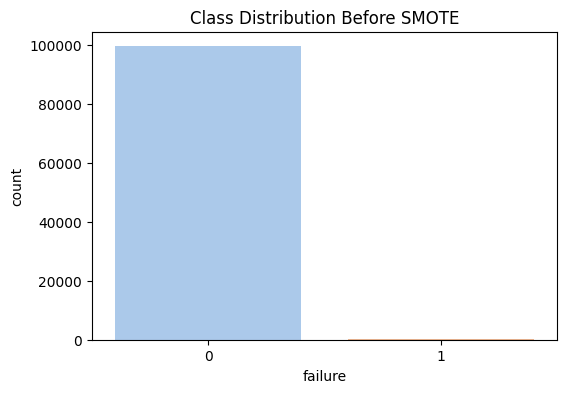
\includegraphics[width=0.8\textwidth]{./figures_akash/before_smote.png} % Replace with your image filename
		\caption{Class Distribution Before SMOTE}
		\label{fig:before_smote}
	\end{figure}
	
	\begin{figure}[h!]
		\centering
		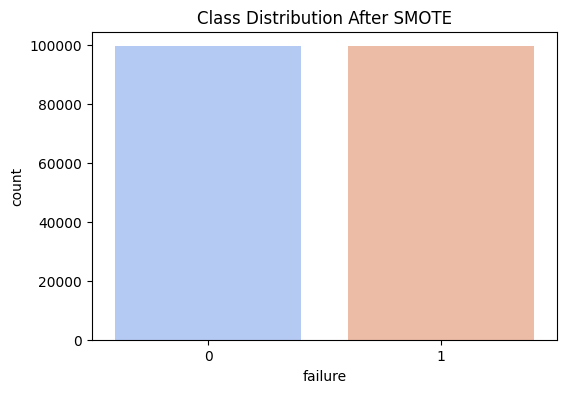
\includegraphics[width=0.8\textwidth]{./figures_akash/after_smote.png} % Replace with your image filename
		\caption{Class Distribution After SMOTE}
		\label{fig:after_smote}
	\end{figure}
	
	\subsection{Evaluation Metrics Visualization}
	The evaluation metrics of the model are visualized in Figure \ref{fig:evaluation_metrics}, highlighting key metrics such as accuracy, precision, recall, and F1-score. This graphical representation provides insight into the model's overall performance.
	
	\begin{figure}[h!]
		\centering
		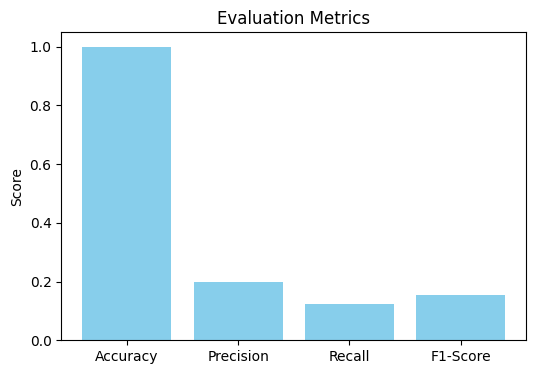
\includegraphics[width=0.75\textwidth]{./figures_akash/evaluation_metrics.png} % Replace with your image filename
		\caption{Evaluation Metrics Visualization}
		\label{fig:evaluation_metrics}
	\end{figure}
	
	\subsection{Confusion Matrix}
	The confusion matrix displayed in Figure \ref{fig:confusion_matrix} represents the model's classification performance by showing the number of true positives, true negatives, false positives, and false negatives.
	
	\begin{figure}[h!]
		\centering
		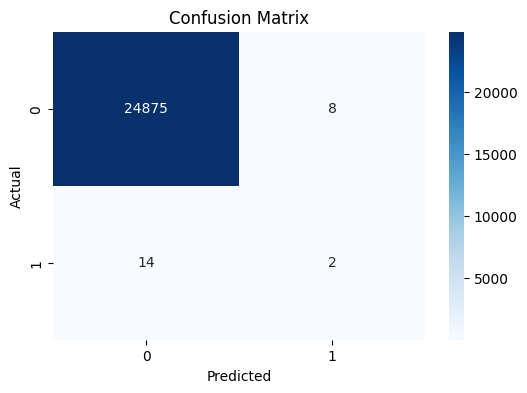
\includegraphics[width=0.75\textwidth]{./figures_akash/confusion_matrix.png} % Replace with your image filename
		\caption{Confusion Matrix}
		\label{fig:confusion_matrix}
	\end{figure}
	
	\section{Conclusion}
	The model performed satisfactorily, achieving balanced metrics after applying SMOTE to address the significant class imbalance in the dataset. The use of SMOTE played a crucial role in enabling the model to better learn from the minority class, leading to improved classification performance.
	
	Efforts were made to tune the hyperparameters of the Random Forest Classifier using methods like GridSearchCV and RandomizedSearchCV. However, due to the large size of the dataset (1 lakh rows and 12 columns), the process proved computationally intensive and caused system limitations. As a result, hyperparameter tuning could not be completed successfully.
	
	Despite these challenges, the model demonstrated reasonable performance using default hyperparameters. Future work could focus on optimizing hyperparameters using more efficient computing resources and exploring advanced algorithms like XGBoost, which are known for their scalability and robust performance on large datasets. Additionally, further feature engineering and model evaluation could enhance the predictive capabilities of the system.
	
	This report highlights the potential and challenges of applying machine learning to predictive maintenance tasks and provides a strong foundation for subsequent refinements.
